\documentclass[tikz,border=6pt]{standalone}
\usepackage{amsmath,amssymb}
\usepackage{xcolor}
\definecolor{accent}{HTML}{A13D2C}
\definecolor{accent2}{HTML}{2B5F6B}
\definecolor{muted}{HTML}{5A564F}
\definecolor{panel}{HTML}{F8F6F0}
\definecolor{linecol}{HTML}{D8D2C4}
\definecolor{astroblue}{HTML}{1B4F72}
\definecolor{sunyellow}{HTML}{E8A33D}
\definecolor{colthree}{RGB}{60,140,80}
\usetikzlibrary{calc,arrows.meta}
\usepackage[T1]{fontenc}\usepackage{newpxtext,newpxmath}  % same fonts as the notes
\begin{document}
% Thermal bremsstrahlung, 4 pi j_nu proportional to T^{-1/2} exp(-h nu/k_B T) at fixed n_e n_i, for k_BT = 2 keV and 8 keV.
% x axis: log10(h nu / keV) from -1 to 1.7; y axis: log10 of j_nu relative to its low-frequency value at k_BT = 2 keV.
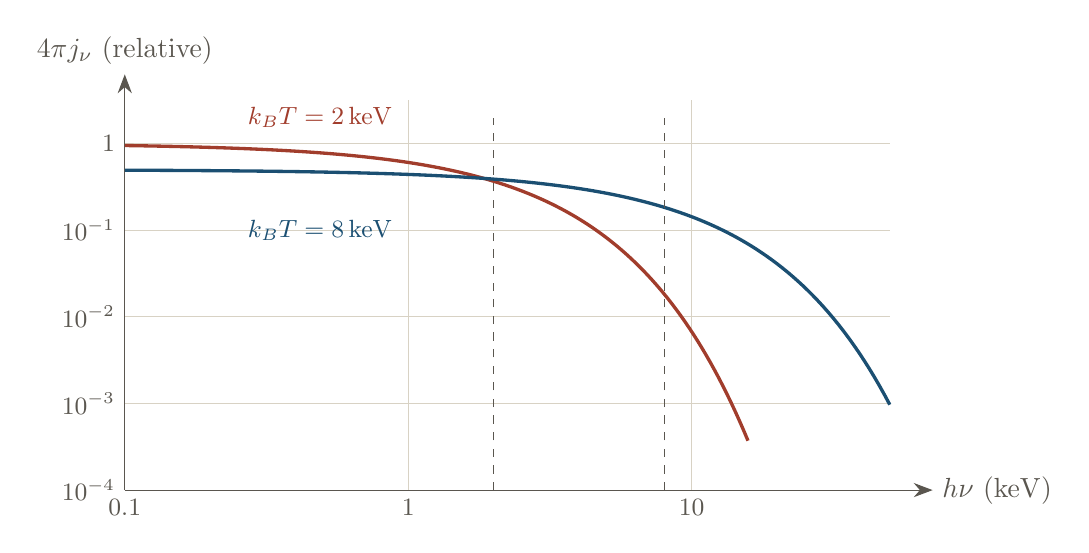
\begin{tikzpicture}[x=3.6cm,y=1.1cm, >={Stealth[length=2.4mm]}]
  \draw[linecol] (-1,-4) grid[xstep=1,ystep=1] (1.7,0.5);
  \draw[->, muted] (-1,-4) -- (1.85,-4) node[right] {$h\nu\ (\mathrm{keV})$};
  \draw[->, muted] (-1,-4) -- (-1,0.8) node[above] {$4\pi j_\nu$ (relative)};
  \foreach \x/\l in {-1/0.1,0/1,1/10} \node[below, muted] at (\x,-4) {\small \l};
  \foreach \y/\l in {-4/{10^{-4}},-3/{10^{-3}},-2/{10^{-2}},-1/{10^{-1}},0/1} \node[left, muted] at (-1,\y) {\small $\l$};
  % log10 j = -0.5 log10(kT/2) - (10^x / kT) log10(e)
  \draw[accent, line width=1.2pt, domain=-1:1.20, samples=150] plot (\x, {-0.5*log10(2/2) - (exp(\x*2.302585)/2)*0.4342945});
  \draw[astroblue, line width=1.2pt, domain=-1:1.70, samples=150] plot (\x, {-0.5*log10(8/2) - (exp(\x*2.302585)/8)*0.4342945});
  \draw[dashed, muted] ({log10(2)},-4) -- ({log10(2)},0.3);
  \draw[dashed, muted] ({log10(8)},-4) -- ({log10(8)},0.3);
  \node[accent, right] at (-0.6,0.3) {\small $k_BT=2\,\mathrm{keV}$};
  \node[astroblue, right] at (-0.6,-1.0) {\small $k_BT=8\,\mathrm{keV}$};
\end{tikzpicture}
\end{document}
